\section{Related Work}
\subsection{Neural Architecture Search (NAS)}
NAS aims to automatically discover optimal neural network architectures from predefined search spaces. NAS methods have achieved impressive success across various tasks. 
Early approaches relied on reinforcement learning~\cite{williams1992simple,pham2018efficient}, evolutionary strategies~\cite{real2019regularized} and Bayesian optimisation~\cite{kandasamy2018neural} to explore the search space.
More recent methods have shifted towards weight sharing techniques. These approaches~\cite{liu2018darts,dong2019one,hu2020dsnas,xu2019pc,xie2018snas,zhang2021idarts,dong2019searching,chen2020drnas,ye2022b} train a single super-network, enabling efficient exploration of various sub-networks (architectures) within the search space.
However, these methods often rely on predetermined search spaces, which limits their ability to discover truly novel architectures. In contrast, our approach addresses the Neural Architecture Design (NAD) task, which is not restricted by predetermined search spaces.

\subsection{LLM Agents}
As large language models have demonstrated impressive
emergent capabilities and have gained immense popularity, recent research has focused on LLM-based autonomous agents to solve complex problems~\cite{xi2023rise}. 
These agents utilize the foundational capabilities of LLMs, displaying remarkable skills in memory~\cite{park2023generative}, planning~\cite{liu2023bolaa}, tool use~\cite{schick2024toolformer,qin2023toolllm}, and reflection~\cite{shinn2024reflexion,zhao2024expel}.
Systems like Visual ChatGPT~\cite{wu2023visual} and HuggingGPT~\cite{shen2024hugginggpt} employ LLMs to orchestrate diverse AI models for complex tasks. Visual programming approaches like~\cite{gupta2023visual} utilize LLMs to generate programs for solving visual tasks based on natural language instructions. 
There are also studies on multi-agent communication~\cite{liang2023encouraging} and collaboration~\cite{hong2023metagpt,qian2023communicative,chen2023agentverse}. For example, MetaGPT~\cite{hong2023metagpt} utilizes an assembly line paradigm, assigning roles to LLM-based agents for collaborative problem-solving.
Our work extends this concept by introducing a team of specialized LLM agents for neural architecture design. 
\begin{figure*}[t]
    \centering
    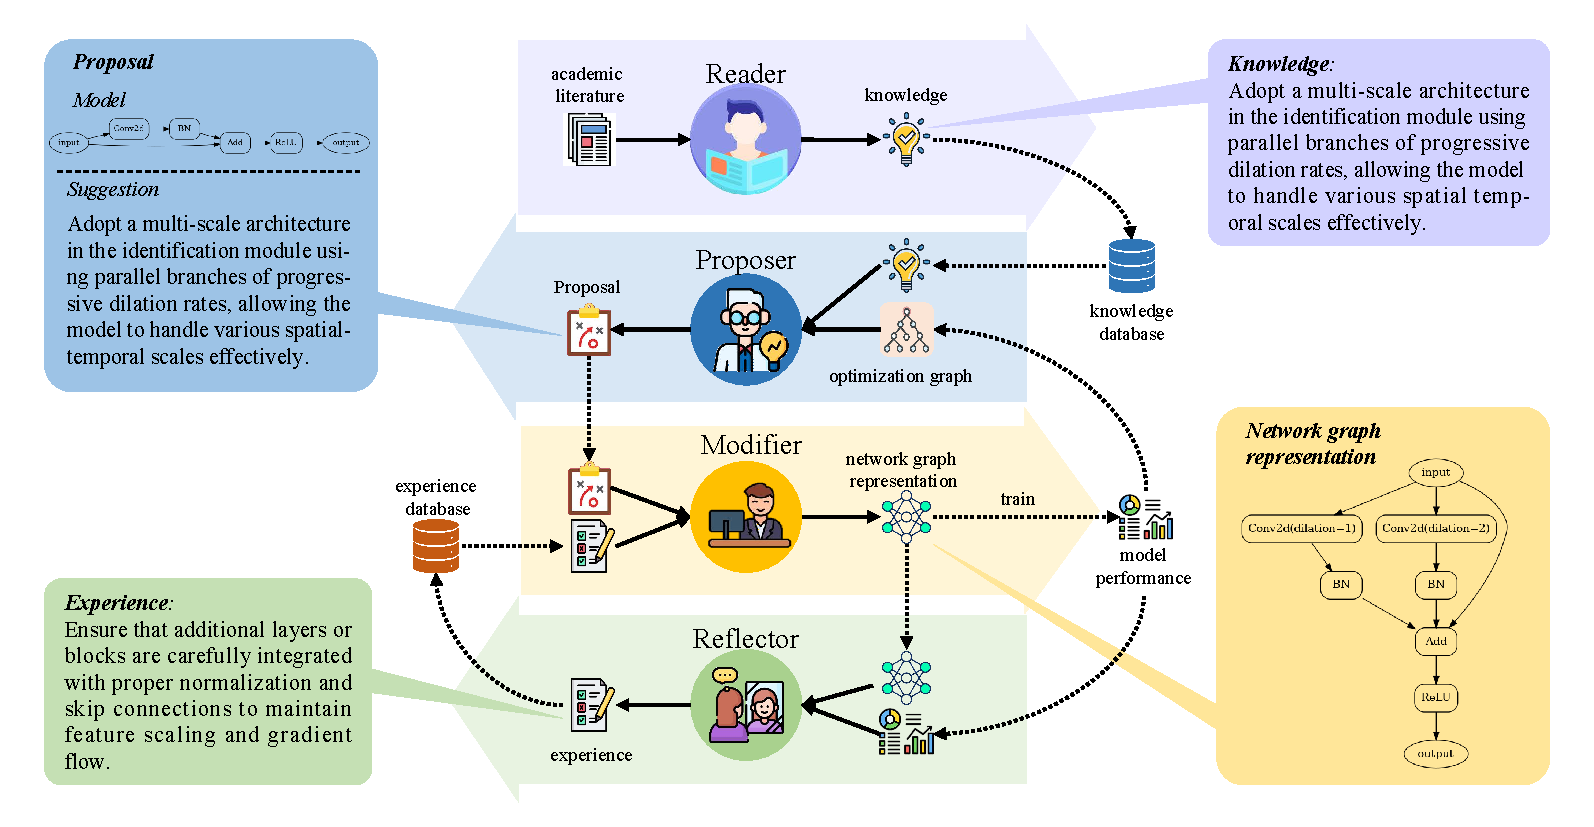
\includegraphics[width=0.99\textwidth]{figures/nader-framework.pdf}
    \caption{Overview of NADER framework. The Reader continuously learns from academic literature, while the Proposer identifies the most promising candidate networks and suggests modifications. The Modifier implements these suggestions, and the Reflector analyzes and provides feedback on the results. The performance of the modified network is relayed back to the Proposer, informing subsequent proposals and fostering a continuous cycle of improvement.}
    \label{fig:framework}
\end{figure*}
\subsection{LLMs for NAS}
Emerging research explores the use of LLMs for NAS. 
GENIUS~\cite{zheng2023can} is a LLM-based NAS algorithm that adopts a straightforward prompt-based search process that prompts GPT-4 to propose designs from a given search space with a handful of examples.
EvoPrompting~\cite{chen2024evoprompting} utilizes code-LLMs as mutation and crossover operators for an evolutionary neural architecture search (NAS) algorithm. 
LLMatic~\cite{nasir2023llmatic} extends EvoPrompting by introducing quality diversity algorithms to discover diverse and robust solutions.
Our work differentiates them by introducing a multi-agent framework, allowing for a more sophisticated and collaborative exploration of the search space. 

